\section{Results}
\subsection{Off-target verification of detection and alarm logic}
All 27 off-target checks passed. Over 96 synthetic records (3.2\,h; 40--180\,bpm; R amplitude 0.55--4.4\,mV) QRS sensitivity was 99.87\,\% (23 of 18\,252 beats missed) and positive predictivity 100\,\%; the worst four-beat heart-rate error was 4.7\,\%. Asystole was annunciated in all 180 episodes, between 4.088 and 4.132\,s after the last R wave, and in all 20 episodes with 0.05\,mV rms noise. When the ECG was reconnected to a patient already in asystole, so that thresholds were learnt on noise alone, the alarm followed within 6.80\,s in all 20 cases. Maximum times to alarm were 2.40\,s for tachycardia, 7.64\,s for bradycardia, 6.98\,s for \texttt{DESAT}, 12.22\,s for \texttt{SPO2\_LOW} and 7.59\,s for \texttt{LOW\_PERF}; leads-off was declared within one sample of the specified 0.5\,s, with no secondary alarm and full detector recovery. SpO$_2$ error was at most 0.7 percentage points over 70--100\,\%. No alarm of any kind occurred in 4\,h of normal rhythm. These figures describe the algorithms on the synthetic source only.

The suite found two defects during development that a demonstration run would not have revealed: the search-back rule accepted the T wave of the last beat before a pause, delaying one asystole alarm in 180 to 4.59\,s (limit 4.5\,s), and the signal source truncated a P wave at the transition into asystole, which the detector counted as a beat. Both were corrected (the first in the detector, the second in the source) and the corresponding checks are retained as regression tests.

\subsection{Alarm latency}
\begin{table}[t]
\caption{Alarm-system latency $L$ in microseconds (three 100\,s runs per configuration). FP: fixed-priority scheduling with priority inheritance and locked memory; TS: time-sharing. Violations are alarms with $L>10$\,ms; the last column is the one-sided 95\,\% upper confidence bound on the violation probability.}
\label{tab:latency}
\small
\begin{tabular}{@{}lrrrrrrrr@{}}
\toprule
Configuration & $n$ & Median & Mean & $P_{99}$ & $P_{99.9}$ & Max & Violations & 95\,\% UB\\
\midrule
\rawinput{tables/tab_latency.tex}
\bottomrule
\end{tabular}
\end{table}

\begin{figure}[t]
\centering
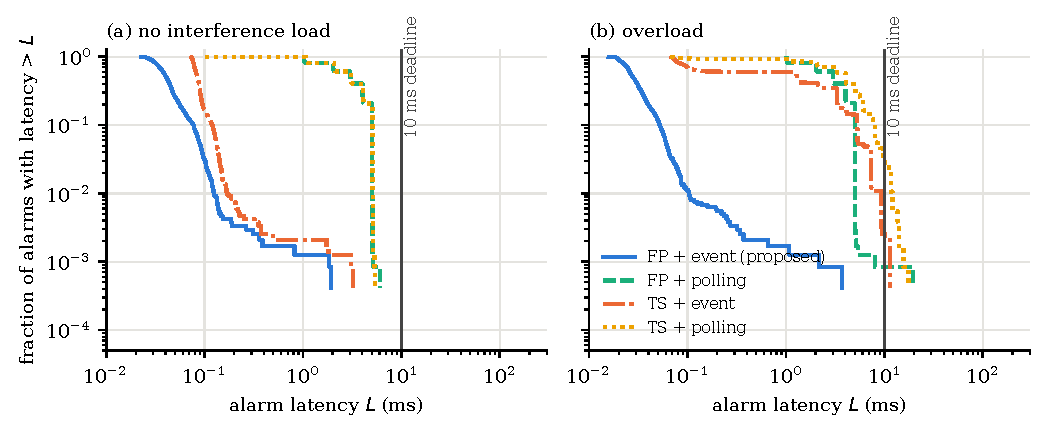
\includegraphics[width=\textwidth]{figs/fig_latency_ccdf.pdf}
\caption{Complementary cumulative distribution of alarm latency for the four architectures, (a) without and (b) with interference load; \NFpEvStrN{} alarms per curve. The plateau of the polled variants reflects the 5\,ms polling period.}
\label{fig:ccdf}
\end{figure}

Table~\ref{tab:latency} and Fig.~\ref{fig:ccdf} summarise \NFpEvStrN{} alarms per configuration. Without load, both event-driven designs had median latencies below 0.1\,ms (\NFpEvIdleMed\,\textmu s for FP, \NTsEvIdleMed\,\textmu s for TS) and no configuration violated the deadline. The polled designs had a median of about 3\,ms and a 99.9th percentile of about 5\,ms, as the polling period predicts.

Under overload the designs separated. With TS scheduling the median latency of the event-driven path rose from \NTsEvIdleMed\,\textmu s to \NTsEvStrMed\,\textmu s, the 99.9th percentile to \NTsEvStrPNNN\,\textmu s, and \NTsEvStrMiss{} alarms (\NTsEvStrMissPct\,\%) violated the deadline; with polling added, \NTsPoStrMiss{} alarms (\NTsPoStrMissPct\,\%) did. With FP scheduling the event-driven path was unaffected in the body of the distribution: the median was \NFpEvStrMed\,\textmu s, the 99.9th percentile \NFpEvStrPNNN\,\textmu s and the maximum \NFpEvStrMaxMs\,ms, with no violation (upper bound \NFpEvStrUB\,\%). The difference between TS and FP event-driven latency under overload was large (Cliff's $\delta=\NTestPolicyDelta$, $p\NTestPolicyP$). The median FP latency was in fact lower under overload than without it (\NFpEvStrMed{} versus \NFpEvIdleMed\,\textmu s, $\delta=\NTestLoadDelta$), which we attribute to the processor not entering an idle state between samples when other threads are runnable.

Fixed-priority scheduling did not, however, make the polled path safe: three of its \NFpPoStrN{} alarms violated the deadline, the worst at \NFpPoStrMaxMs\,ms. Polling consumes half of the 10\,ms budget by construction, so a platform stall of 5\,ms or more, which the next subsection shows does occur, is enough for a violation. The event-driven path keeps almost the whole budget in reserve for such stalls.

\subsection{Release jitter and per-sample pipeline latency}
\begin{table}[t]
\caption{Acquisition release jitter and pipeline latency (nominal release to end of processing) in microseconds over all samples of the probe runs, and the number of samples whose pipeline latency exceeded the 10\,ms alarm budget.}
\label{tab:jitter}
\small
\begin{tabular}{@{}lrrrrrrrr@{}}
\toprule
 & & \multicolumn{3}{c}{Release jitter} & \multicolumn{3}{c}{Pipeline latency} & \\
\cmidrule(lr){3-5}\cmidrule(lr){6-8}
Configuration & Samples & Median & $P_{99.9}$ & Max & Median & $P_{99.9}$ & Max & $>$10\,ms\\
\midrule
\rawinput{tables/tab_jitter.tex}
\bottomrule
\end{tabular}
\end{table}

\begin{figure}[t]
\centering
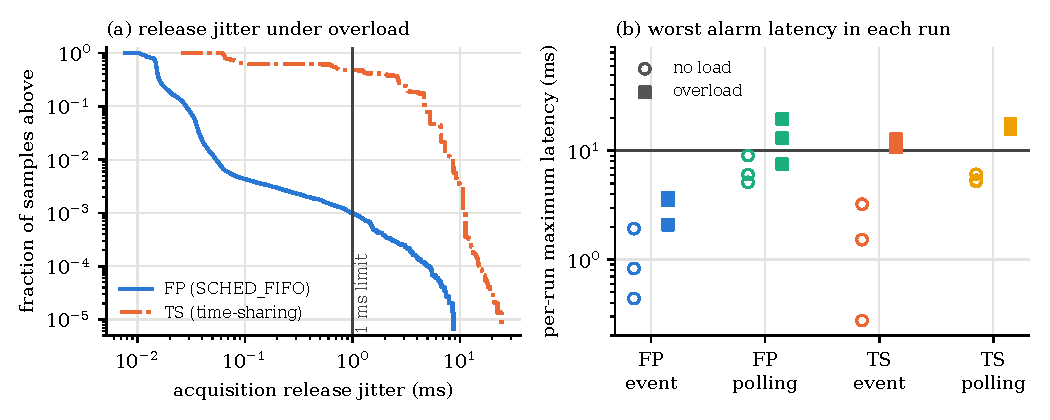
\includegraphics[width=\textwidth]{figs/fig_jitter.pdf}
\caption{(a) Complementary cumulative distribution of acquisition release jitter under overload for fixed-priority and time-sharing scheduling (event-driven path, \NFpEvStrNSamp{} samples each). (b) Largest alarm latency observed in each of the 24 probe runs; the horizontal line is the 10\,ms deadline.}
\label{fig:jitter}
\end{figure}

An alarm can become true on any sample, so the latency of every sample is a stricter test than the latency of the alarms that happened to be injected. Table~\ref{tab:jitter} reports it for \NFpEvStrNSamp{} samples per configuration. Under overload with TS scheduling, \NTsEvStrJitOver{} samples (48\,\%) were released more than 1\,ms late and \NTsEvStrPipeMiss{} (\NTsEvStrPipeMissPpm{} per million) completed processing more than 10\,ms after their nominal release. With FP scheduling the corresponding numbers were \NFpEvStrJitOver{} samples above 1\,ms and \NFpEvStrPipeMiss{} sample above 10\,ms (\NFpEvStrPipeMaxMs\,ms), a reduction by more than two orders of magnitude, but not to zero.

That single sample, and release jitter of up to \NFpEvStrJitMaxMs\,ms at real-time priority (\NFpPoStrJitMaxMs\,ms in the FP polled runs), are the central negative result. Jitter of several milliseconds also occurred without any load (maximum \NFpEvIdleJitMaxMs\,ms, \NFpEvIdleJitOver{} samples above 1\,ms), in a thread that had the highest priority on its processor and nothing to compete with. Requirement SRS-RT-04 (jitter $\le 1$\,ms) therefore failed in every configuration, and the per-sample form of SRS-RT-01 failed for the proposed configuration by one sample in \NFpEvStrNSamp. No sample or alarm event was lost in any run.

\subsection{Measured latency against the application-level bound}
\begin{table}[t]
\caption{Execution times observed with the per-thread CPU-time clock in the proposed configuration under overload, and terms of Eqs.~\eqref{eq:rta}--\eqref{eq:bound}. $C_{\mathrm{wdg}}$ and $B$ come from a supplementary overload run with two additional probes.}
\label{tab:rta}
\small
\begin{tabular}{@{}lr@{}}
\toprule
Quantity & Value (\textmu s)\\
\midrule
$C_{\mathrm{acq}}$: mean / 99.99th percentile / maximum & \NWcCacqmean{} / \NWcCacqpq{} / \NWcCacq\\
$C_{\mathrm{proc}}$: mean / 99.99th percentile / maximum & \NWcCprocmean{} / \NWcCprocpq{} / \NWcCproc\\
$C_{\mathrm{alm}}$: maximum & \NWcCalarm\\
$C_{\mathrm{wdg}}$: maximum & \NWcCwdg\\
$B$ (display critical section): maximum & \NWcBui\\
\midrule
$R_{\mathrm{app}}$ from Eq.~\eqref{eq:rta} with observed maxima, $m=1$ & \NWcRapp\\
Largest $L$ minus release jitter of the triggering sample & \NWcresidmax\\
Largest alarm latency $L$ & \NWcLmax\\
Largest release jitter & \NWcjitmax\\
\bottomrule
\end{tabular}
\end{table}

Table~\ref{tab:rta} places these observations in the terms of Section~\ref{sec:rta}. The mean processor demand of acquisition plus processing was about \NWcCacqmean\,+\,\NWcCprocmean\,\textmu s per 2\,000\,\textmu s period, a utilisation of \NWcUtil\,\%. Observed maxima were two orders of magnitude above the means; maxima of this kind on a virtual machine probably include time in which the thread was charged but not running, and we use them as conservative inputs. They give $R_{\mathrm{app}}=\NWcRapp$\,\textmu s, well inside one sampling period. The supplementary run that supplied $C_{\mathrm{wdg}}$ and $B$ (100\,s, 2\,350 alarms, not included in Table~\ref{tab:latency}) had a larger maximum alarm latency than any campaign run, 7.57\,ms, still without a deadline violation; this illustrates how much an observed maximum depends on the observation window.

To compare with measurement we subtracted from each alarm latency the release jitter of its triggering sample, leaving the time from the actual start of acquisition to annunciation. Under overload this residual had a median of \NFpEvStrResP\,\textmu s, a 99.9th percentile of \NFpEvStrResPNNN\,\textmu s and a maximum of \NWcresidmax\,\textmu s, within $R_{\mathrm{app}}$. Of the \NFpEvStrNGtOne{} alarms with $L>1$\,ms, late release accounted on average for \NFpEvStrLateShare\,\% of the latency. In other words, once the acquisition thread ran, the architecture delivered the alarm within the analysed bound; what the bound does not cover, the term $\Lambda$, was up to \NFpEvStrJitMaxMs\,ms and dominated every long latency. (Without load, two alarms had residuals above $R_{\mathrm{app}}$, up to \NFpEvIdleResMax\,\textmu s, which shows that stalls also strike after release.)

\subsection{Watchdog fault injection}
\begin{table}[t]
\caption{Time from the start of an injected 400\,ms runaway loop in the processing thread to annunciation of \texttt{SYS\_STALL}, under overload (requirement: $\le 200$\,ms).}
\label{tab:stall}
\small
\begin{tabular}{@{}lrrrrr@{}}
\toprule
Configuration & Runs & Undetected & Min (ms) & Mean (ms) & Max (ms)\\
\midrule
\rawinput{tables/tab_stall.tex}
\bottomrule
\end{tabular}
\end{table}
The watchdog detected every injected stall (Table~\ref{tab:stall}), in at most \NFpStallMax\,ms with FP scheduling, consistent with five 20\,ms checks plus up to one period of phase. With FP scheduling the watchdog and alarm manager pre-empt the runaway thread by priority; with TS scheduling detection relied on the fairness of the scheduler and was also timely in these runs, with one detection slightly below 100\,ms because the processing thread had already been starved before the fault was injected.

\subsection{Clinical scenario in real time}
\begin{table}[t]
\caption{Alarms raised in the 210\,s clinical scenario executed in real time: algorithmic delay $A$ from the reference instant, for three runs with FP scheduling (one without load, two under overload; range) and one run with TS scheduling under overload.}
\label{tab:clinical}
\small
\begin{tabular}{@{}llllll@{}}
\toprule
Alarm & Priority & Reference & $A$, FP (s) & $A$, TS (s) & Limit (s)\\
\midrule
\rawinput{tables/tab_clinical.tex}
\bottomrule
\end{tabular}
\end{table}

\begin{figure}[t]
\centering
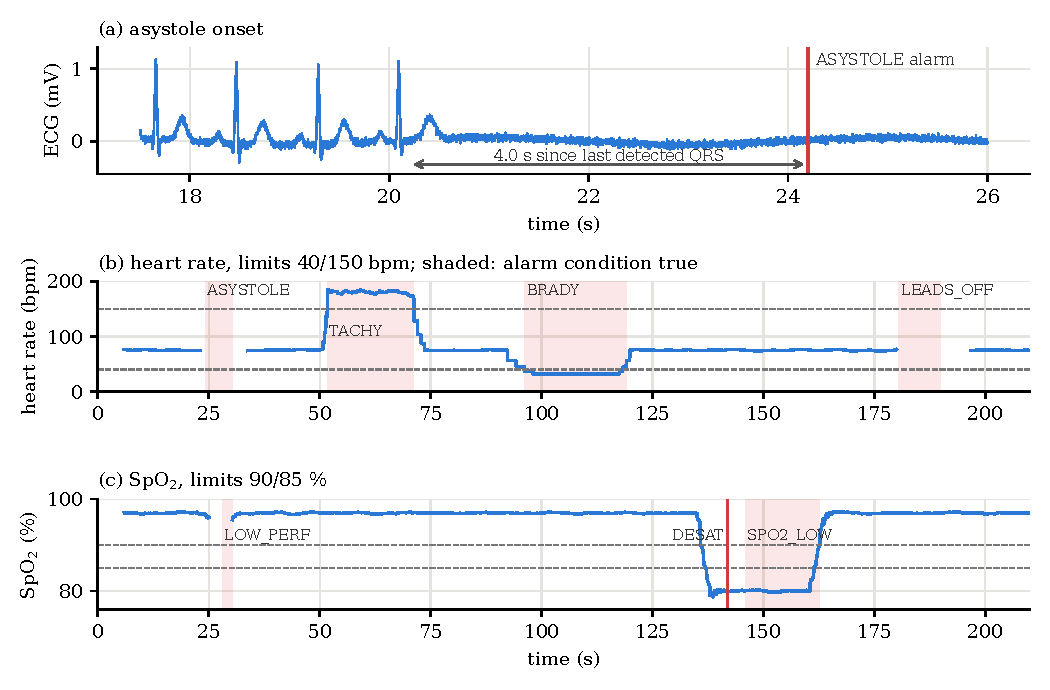
\includegraphics[width=\textwidth]{figs/fig_clinical.pdf}
\caption{Clinical scenario (off-target trace of the same code): (a) ECG at the onset of asystole; (b) heart rate and (c) SpO$_2$ with the intervals in which alarm conditions were true.}
\label{fig:clinical}
\end{figure}

In each real-time run of the clinical scenario exactly the seven expected alarms were raised, once each, with the algorithmic delays of Table~\ref{tab:clinical}; Fig.~\ref{fig:clinical} shows the scenario. Because persistence timers count samples, the TS run raised every alarm on exactly the same sample as the FP run that used the same random seed: scheduling changes when an alarm is annunciated, not whether or on which sample it is raised. The alarm-system latency of the \NClinFpN{} alarms in the FP runs was at most \NClinFpLatMax\,\textmu s; in the TS run under overload it reached \NClinTsLatMaxMs\,ms.

\subsection{Traceability status}
Of the \NVerTotal{} automated checks, \NVerPass{} passed and \NVerFail{} failed (\NFailList). Because status propagates along the links, \NHazOpen{} of the \NHaz{} hazards are reported as open in Table~\ref{tab:hazard}: those whose control depends on bounded alarm latency or on bounded release jitter. All \NHazUnaccInit{} hazards rated unacceptable before controls are rated tolerable or acceptable after them, on the condition that the open items are closed on a platform with a bounded $\Lambda$.

\section{Discussion}
\subsection{What the comparison shows}
Three observations follow from the experiment. First, the cost of the processing itself is irrelevant to alarm latency: QRS detection, SpO$_2$ estimation and alarm evaluation together need about two microseconds per sample on this processor, a utilisation of \NWcUtil\,\%. Any latency problem in a monitor of this kind is a scheduling problem. Second, the scheduling class decides the outcome under overload. With time-sharing, nearly half of all samples were acquired more than a millisecond late and one alarm in four hundred missed a 10\,ms deadline, although the monitor's own demand was negligible; with fixed priorities, priority inheritance and locked memory the body of the latency distribution did not move at all. Time-sharing schedulers optimise fairness and throughput, and a design that relies on them inherits the behaviour of whatever else is installed on the device. Third, the alarm path matters independently of the scheduler. A polled alarm manager spends a fixed part of the budget on waiting, and it was the only fixed-priority variant whose alarms violated the deadline.

\subsection{What a measurement on a general-purpose kernel can and cannot support}
We set out to verify a hard deadline and must report that, on the evaluation platform, we could not. No alarm of the proposed configuration was late, and the upper confidence bound on the violation probability is \NFpEvStrUB\,\%; but one sample in \NFpEvStrNSamp{} was processed after the deadline, and release jitter reached \NFpEvStrJitMaxMs\,ms. Had an alarm condition become true on that sample, the requirement would have been violated. The decomposition of Table~\ref{tab:rta} locates the cause outside the application: the time from the actual start of acquisition to annunciation stayed within the analysed bound, and long latencies were explained by late release. The same stalls appeared without load, which points to the hypervisor and the non-real-time kernel rather than to the interference threads. The guest kernel's own accounting supports the first explanation: it reported about 45\,s of processor time stolen by the hypervisor, summed over the four virtual processors, during the hour of the campaign. We cannot apportion individual stalls between hypervisor and kernel with the instrumentation used here.

This is the argument for a real-time operating system, stated as a measurement rather than as an assumption. The application-level bound $R_{\mathrm{app}}$ becomes a guarantee only when the platform term $\Lambda$ is bounded by construction and by evidence from the supplier, which is what a microkernel such as QNX Neutrino \cite{hildebrand1992}, or \texttt{PREEMPT\_RT} with a kernel-level analysis \cite{bristot2020}, is meant to provide. Our results neither confirm nor quantify that for QNX. They do show that the software is ready for the experiment: the same binaries, scripts and hazard log will report, on a bare-metal real-time target, whether the open items close. We regard the fact that the generated hazard log currently reports \NHazOpen{} open hazards as a feature of the method. A traceability report assembled by hand after the fact would very likely have recorded the zero late alarms and passed.

\subsection{Hazard-driven design}
The hazard analysis changed the software in ways that functional testing alone would not have prompted. The threshold floor, the exclusion of the T-wave window from search-back, the perfusion gate on SpO$_2$ and the re-learning after lead reconnection are each a response to a specific hazardous situation, and each has a test that fails without it. The reverse also held: a verification test for one hazard (asystole time-to-alarm) exposed a defect in a mechanism introduced for another purpose (search-back for missed beats). Keeping the links as data and regenerating the report from executed results cost a few hundred lines of script and addresses the maintenance problem reported for traceability in practice \cite{regan2013}, at least at this scale.

\subsection{Limitations}
\begin{itemize}
\item \emph{Platform.} All timing results come from a virtualised, non-real-time Linux kernel on a shared host, with light unrelated activity on another virtual processor during the campaign. Absolute values will not transfer to other hardware. No measurement was made on QNX; the port has not been compiled.
\item \emph{Duration.} Each configuration was observed for 300\,s. Worst-case behaviour of an operating system emerges over hours or days and under a wider range of loads (interrupt storms, network traffic, storage errors); the maxima reported here are lower bounds on the worst case.
\item \emph{Timing source.} Latencies were measured with the system's own monotonic clock. A stall that also stops the clock source, or an error in the annunciator device itself, is invisible; an external logic analyser on a hardware output is the appropriate reference.
\item \emph{Execution times.} $C$ values are observed maxima, not results of static worst-case execution-time analysis, and include virtualisation artefacts.
\item \emph{Signals and algorithms.} The ECG and photoplethysmogram are synthetic and free of motion artefact, ectopy, pacing and morphology changes; detection figures say nothing about performance on patients. Ventricular fibrillation and tachycardia are not classified, there is one ECG lead, and the SpO$_2$ calibration is the textbook linear curve. Evaluation on annotated databases \cite{goldberger2000,moody2001,clifford2015} is required before any clinical claim.
\item \emph{Alarm system.} Audio pause, alarm limits configurable by the operator, distributed alarm systems and the human factors of annunciation are not implemented. A single-core analysis was used; multi-core deployments need partitioned or global analysis.
\item \emph{Risk analysis.} The hazard log was produced by engineering judgement without clinical or regulatory review. It illustrates a method and is not a risk-management file.
\end{itemize}

\subsection{Future work}
The immediate next step is to repeat the campaign unchanged on QNX Neutrino and on a \texttt{PREEMPT\_RT} kernel on the same single-board computer, with an external timing reference and runs of at least 24\,h, and to replace the synthetic source by replay of annotated recordings. The thread structure also offers a natural place for computationally heavy, non-critical analysis such as learned ECG interpretation or language-model summarisation of alarm context: in the time-sharing class next to the display thread, where the present results indicate that it cannot delay the alarm path provided the scheduling and synchronisation rules of Section~3 are kept. Quantifying that isolation with a realistic inference workload is a direct extension of the overload experiment.

\section{Conclusion}
We built a patient-monitor simulator in which the software contribution to alarm delay is defined, analysed, linked to a hazard log and measured for every alarm. On a general-purpose kernel under CPU, memory and I/O overload, fixed-priority scheduling with an event-driven alarm path kept the median alarm latency at \NFpEvStrMed\,\textmu s and all \NFpEvStrN{} alarms within the 10\,ms deadline, where the time-sharing equivalent violated it in \NTsEvStrMissPct\,\% of alarms and a polled fixed-priority design in three. The same measurements show that the platform, not the application, sets the worst case: one sample in \NFpEvStrNSamp{} exceeded the budget and release jitter reached \NFpEvStrJitMaxMs\,ms, so the corresponding requirements are reported as failed and their hazards as open. The released code, hazard log and measurement harness allow that verdict to be re-evaluated on a real-time operating system without modification.
